%%%%%%%%%%%%%%%%%%%%%%%%%%%%%%%%%%%%%%%%%%%%%%%%%%%%%%%%%%%%%%%%%%%%%%%%%%%%%%%%
%2345678901234567890123456789012345678901234567890123456789012345678901234567890
%        1         2         3         4         5         6         7         8

%\documentclass[letterpaper, 10 pt, conference]{ieeeconf}  % Comment this line out
                                                          % if you need a4paper
\documentclass[a4paper, 10pt, conference]{ieeeconf}      % Use this line for a4
                                                          % paper

\IEEEoverridecommandlockouts                              % This command is only
                                                          % needed if you want to
                                                          % use the \thanks command
\overrideIEEEmargins
% See the \addtolength command later in the file to balance the column lengths
% on the last page of the document


\let\labelindent\relax

% The following packages can be found on http:\\www.ctan.org
\usepackage{graphics} % for pdf, bitmapped graphics files
\usepackage{epsfig} % for postscript graphics files
%\usepackage{mathptmx} % assumes new font selection scheme installed
%\usepackage{times} % assumes new font selection scheme installed
\usepackage{amsmath} % assumes amsmath package installed
\usepackage{amssymb}  % assumes amsmath package installed
\let\proof\relax
\let\endproof\relax
\usepackage{amsthm}

\usepackage{url}
\usepackage[ruled, vlined, linesnumbered]{algorithm2e}
%\usepackage{algorithm}
\usepackage{verbatim} 
%\usepackage[noend]{algpseudocode}
\usepackage{soul, color}
\usepackage{lmodern}
\usepackage{fancyhdr}
\usepackage[utf8]{inputenc}
\usepackage{fourier} 
\usepackage{array}
\usepackage{makecell}
\usepackage[inline]{enumitem}
\usepackage{url}
\usepackage{subcaption} 
\usepackage{hyperref}
\usepackage{dblfloatfix}
\usepackage[british]{babel}
\usepackage[sorting=none, style=ieee, bibstyle=ieee, backend=biber, citestyle=numeric-comp]{biblatex}
\addbibresource{reference.bib}



\theoremstyle{plain}
\newtheorem{thm}{Theorem}[section] % reset theorem numbering for each chapter
\theoremstyle{definition}
\newtheorem{nota}[thm]{Notation}
\newtheorem{defn}[thm]{Definition} % definition numbers are dependent on theorem numbers
\newtheorem{exmp}[thm]{Example} % same for example numbers
\newtheorem{hyp}{Hypothesis}



\SetNlSty{large}{}{:}

\renewcommand\theadalign{bc}
\renewcommand\theadfont{\bfseries}
\renewcommand\theadgape{\Gape[4pt]}
\renewcommand\cellgape{\Gape[4pt]}

\newcommand{\rework}[1]{\todo[color=yellow,inline]{#1}}

\makeatletter
\newcommand{\rom}[1]{\romannumeral #1}
\newcommand{\Rom}[1]{\expandafter\@slowromancap\romannumeral #1@}
\makeatother

\pagestyle{plain} 

\title{\LARGE \bf
Dynamic Windows Processing in RDF Mapping engines for data streams 
}

%\author{ \parbox{3 in}{\centering Huibert Kwakernaak*
%         \thanks{*Use the $\backslash$thanks command to put information here}\\
%         Faculty of Electrical Engineering, Mathematics and Computer Science\\
%         University of Twente\\
%         7500 AE Enschede, The Netherlands\\
%         {\tt\small h.kwakernaak@autsubmit.com}}
%         \hspace*{ 0.5 in}
%         \parbox{3 in}{ \centering Pradeep Misra**
%         \thanks{**The footnote marks may be inserted manually}\\
%        Department of Electrical Engineering \\
%         Wright State University\\
%         Dayton, OH 45435, USA\\
%         {\tt\small pmisra@cs.wright.edu}}
%}

\author{Sitt Min Oo
\\
\\
Supervisors: Prof.~Dr. Ruben Verborgh and Dr. Anastasia Dimou\\
Counsellor: Gerald Haesendonck
}


\begin{document}



\maketitle
\thispagestyle{plain}
\pagestyle{plain}



%%%%%%%%%%%%%%%%%%%%%%%%%%%%%%%%%%%%%%%%%%%%%%%%%%%%%%%%%%%%%%%%%%%%%%%%%%%%%%%%
%%%%%%%%%%%%%%%%%%%%%%%%%%%%%%%%%%%%%%%%%%%%%%%%%%%%%%%%%%%%%%%%%%%%%%%%%%%%%%%%
\begin{abstract}

Current state-of-the-art approaches mapping non-RDF to RDF data in 
a streaming environment focus more on the efficiency of the 
mapping process with minimal support for multi-stream processing. 
The existing approaches for supporting simple multi-stream 
processing operators in mapping engines are very limited or apply fixed window size.

Therefore, we implemented a dynamic window mechanism in RMLStreamer, which 
adapts its size according to the changing stream characteristics with
negligible memory overhead, low latency, and high throughput. We evaluated the dynamic window
under different workload with varying stream velocity. The results 
show that it achieves latency in the millisecond range, with higher 
throughput than fixed size windows in all workload situations. \\ 
\end{abstract}

\begin{keywords}
RDF, RMLStreamer, RML, Adaptive windows, Dynamic windows,
Stream joins, Multi-stream processing.

\end{keywords}

%%%%%%%%%%%%%%%%%%%%%%%%%%%%%%%%%%%%%%%%%%%%%%%%%%%%%%%%%%%%%%%%%%%%%%%%%%%%%%%%
%%%%%%%%%%%%%%%%%%%%%%%%%%%%%%%%%%%%%%%%%%%%%%%%%%%%%%%%%%%%%%%%%%%%%%%%%%%%%%%%
\section{INTRODUCTION}
\label{chap:intro}

%Heterogeneous data formats, such as CSV or HTML, are not
%designed to semantically enrich the data they represent and 
%machines have difficulty interpreting these data automatically.
Various data formats such as CSV or HTML are not designed to contain the semantics of their data
which avoids machines to automatically interpret these data. 
To ensure that these heterogeneous data format are interpretable and 
processable by machines, data formats based on W3C standards, such as Resource Description 
Framework (RDF) triples~\cite{intro_rdf}, are developed. 
There exist state-of-the-art approaches to consolidate heterogeneous data
and transform them to an RDF serialization in a streaming environment. 

These approaches support traditional stream operators like joins and aggregations. 
However, they do not consider
the characteristics of streaming data sources such as velocity and 
time-correlations between the different
input streams, either due to the 
fixed size windows or custom solutions which they apply. 

Therefore, we propose a dynamic window as a solution to varying characteristics of streaming data. We evaluated our 
approach with the join operator applied inside the window. 
The dynamic window improves the performance of the 
join operator with higher throughput, lower latency and 
similar memory usage compared to a fixed size window.

The source code and the evaluation setup code can be found at
\url{https://github.com/RMLio/RMLStreamer/tree/feature/window_joins}, and 

\href{https://github.com/Kortika/Thesis-test-scripts.git}{https://github.com/Kortika/Thesis-test-scripts.git} respectively.


\section{RELATED WORKS} 
\label{sec:RELATED WORKS} 
There exists state-of-the-arts approaches to map non-RDF data 
to RDF data in a streaming environment. These approaches 
implement diferent strategies when it comes to applying 
multi-stream processing. Furthermore, we will also outline
the existing works on windowing to handle changing characteristics 
of the input data stream. 

\subsection{Mapping implementations}
\subsubsection{SPARQL-Generate} 
SPARQL-Generate~\cite{sparql_generate} 
is based on an extension of SPARQL 1.1 query language, to leverage 
its expressiveness and extensibility. 
It can be implemented on top 
of any existing SPARQL query engine. 
M. Lefran\c{c}ois~\cite{sparql_generate} clarified that when joining
records from two different streams, SPARQL-Generate will fully consume the records 
from the "parent" stream and index it internally in memory first, before 
iteratively consuming the "child" stream for joining. 

\subsubsection{TripleWave} 
TriplWave~\cite{triple_wave}  is based on an extension of 
R2RML to consume heterogeneous data for publication of RDF data. 
Therefore, it only focuses on the mapping of non-RDF data stream to RDF data stream. 
Although it supports simple \emph{join} operator, it does not have a 
dynamic window to handle changing characterisitcs of a data stream.

\subsubsection{RDFGen}
RDF-Gen~\cite{rdf_gen} is based on its own custom syntax 
similar to a combination SPARQL and Turtle syntax. It processes the input 
individually therefore it employs windowing to perform multi stream operator. 
However, since the implementation is closed source, we could not confirm if 
the window is fixed size or dynamic. 

\subsubsection{RMLStreamer}
RMLStreamer~\cite{rml_streamer}
was developed to parallelize the ingestion and mapping process of RDF data generation pipeline. 
It is based on the work of RMLMapper~\cite{rml}, an RDF mapping engine consuming bounded data and mapping them to RDF data with the use of RML. Hence, RMLStreamer can also 
process heterogeneous data and generate RDF data. It does not support 
multi stream operator at this moment, however, the ease of scalability by RMLStreamer
is desirable as a stream mapping engine. 


\subsection{Windows}
Several studies have been conducted to 
improve the join algorithms in windows~\cite{vctw_join, join_tracking, grubjoin, approximate_window_sem, approx_window}. 
The approaches in ~\cite{grubjoin, approximate_window_sem, approx_window} are based 
on dropping some of the records to be joined through \emph{load shedding} if the 
records failed to meet a threshold. These threshold calculation requries 
memory overhead for storing statistical model per window or 
assumption of the stream being in-order for them to work
~\cite{grubjoin, approximate_window_sem, approx_window}.

On the other hand, VC-TWJoin~\cite{vctw_join} considers only the velocity of the 
stream to adjust the window sizes. 
However, the approach is unstable when the data stream has periodic bursts of data.
It either increases or decreases the size of the window when themetric triggers 
the threshold of the algorithm. In the worst-case scenario it 
can lead to cyclic increase and 
decrease of window sizes if the metric borders around the threshold with every 
update of the metric.







\section{DYNAMIC WINDOW}%
\label{sec:Dynamic Window}
A dynamic window is a type of partitioned window~\cite{generic_window_sem}.
We define it as a group of subwindows, which update their sizes dynamically according to the characteristics 
of the data stream. It groups the incoming streams into different partitions first, according to 
the \emph{key} attribute value of the records. Subsequently, these grouped records are assigned 
to individual subwindows. These subwindows adjust their own size independently from each other 
at each update cycle. Furthermore, the subwindows will be independent from each other such 
that the stream rate is local to the attribute value for which each subwindow is responsible. 

\subsection{Dynamic window join}
\label{sub:Dynamic window join}

The join algorithm used, is a variant of Symmetric Hash Join~\cite{symmetric_hash_join}. 
The subwindows themselves work like a hash table, containing records with a 
specific \emph{key} --- since they are \emph{partitioned}. 
The records are joined by probing the relevant stream and generating the 
joined result. 


\subsection{Dynamic window algorithm}%
\label{sub:Dynamic window algorithm}
For each subwindow, the following configuration parameters 
are provided: 

\begin{itemize}
    \item $\Delta n$: the \textbf{initial} interval of time before the next eviction trigger. 
    \item $\epsilon_u$: the upper limit threshold for the total cost metric.
    \item $\epsilon_l$: the lower limit threshold for the total cost metric. 
    \item $U$: the upper limit for the window size. 
    \item $L$: the lower limit for the window size. 
\end{itemize}

Since we are implementing the join operator, the trigger event is fired when current record 
$r_c$ arrives, and the symmetric hash join is executed. We denote the current window as 
$W$ with the size as $|W|$. The streams are denoted as $S_P$ and $S_C$ with 
the corresponding states $List_P$ and $List_C$, for the parent and 
the child stream respectively. The states contain the records from their 
respective streams inside the subwindows.

The eviction trigger is fired every time when the current watermark 
$w \ge |W| + \Delta n$. At each eviction trigger we calculate
the cost for each \emph{list states} $List_P$ and $List_C$, containing the records from $S_P$ and $S_C$
respectively. The cost for $cost(List_P) = |S_P|/Size(List_P)$, idem for $cost(List_C)$. 
The total cost is $m = cost(List_P) + cost(List_C)$ and it is checked against thresholds $\epsilon_l$ and $\epsilon_u$. If  $\epsilon_l \le m \le \epsilon_u$, 
$\Delta n$ stays the same, otherwise it will be adjusted accordingly. This provides some stability 
in window size by keeping the same size if the cost lies within the thresholds. 
The higher $m$, the higher the stream rate. Thus, the subwindow needs to be frequently 
evicted and lower $\Delta n$ to reduce memory usage. There is also a limit on the 
minimum and maximum window sizes, $L$ and $U$ respectively, to ensure that the window 
size $\Delta n$ does not keep growing or shrinking in size infinitely in a worst-case scenario. 
The sizes of the list states 
are also updated according to $Size(List_P) = Size(List_P) * cost(List_P) + 0.5$.
Similarly for $Size(List_C)$. 
Hence the dynamic window maintains an 
ideal size by adjusting $\Delta n, Size(List_P)$ and $Size(List_C)$ according to 
the stream rate. The pseudo code for the eviction algorithm is presented in Algorithm~\ref{alg:dynamic_eviction}.

This algorithm for the dynamic window is an adaptation of the VC-TWindow~\cite{vctw_join} with 
improvements for stability in window sizing, clarity in the metrics used for updates, and localization 
of window size update to each subwindow.  

\begin{algorithm}[htbp]
    \DontPrintSemicolon
    \KwData{$\Delta n, \epsilon_u, \epsilon_l, U, L, List_P, List_C, S_P, S_C$}

    $cost(List_P) = |S_P| / Size(List_P)$      
    
    $cost(List_C) = |S_C| / Size(List_C)$     


    total cost $ m = cost(List_P) + cost(List_C)$  
  
    \If{$m > \epsilon_u$} 
    {
    
        $\Delta n = \Delta n / 2 $ 
        
        $Size(List_P) = Size(List_P) * (cost(List_P) + 0.5)$  

        $Size(List_C) = Size(List_C) * (cost(List_C) + 0.5)$  
    }
    \ElseIf{$m < \epsilon_l$}
    {
   
        $\Delta n = \Delta n * 2$ 

        $Size(List_P) = Size(List_P) * (cost(List_P) + 0.5)$  

        $Size(List_C) = Size(List_C) * (cost(List_C) + 0.5)$  
    }

    clean both $List_C \text{ and } List_P$
    \caption{Dynamic window $onEviction$ routine}
    \label{alg:dynamic_eviction}
\end{algorithm}




\section{IMPLEMENTATION}%
\label{sec:Implementation}

The dynamic window is implemented for RMLStreamer 
to extend its capabilities to do simple stream processing by 
joining multiple streams.  Furthermore, we extended RML
with new ontologies to allow the configuration of the window. 

\subsection{RML ontology extension}
We extended RML to support configuration of window when
joining the \emph{reference object map} with its \emph{parent triples map}. 
Currently, it only supports the rudimentary 
configuration of the type of join to be applied.

\subsection{Dynamic window}
The dynamic window is implemented using Apache Flink's 
\emph{KeyedCoProcessFunction} API with the state management 
done using Flink's \emph{ListStates}.

\section{EVALUATION}
\label{chap:Evaluation}

To measure the effectiveness of dynamic windowing for multi-stream operators during the 
mapping of non-RDF heterogeneous data we need to measure the following 
metrics of our stream processing framework: \emph{CPU usage}, \emph{latency}, \emph{throughput},
\emph{memory usage}, and \emph{completeness}. 

\subsection{Data}
We use the same data 
as the benchmark in the paper by Van Dongen and Van den Poel~\cite{evalution_of_spe}. 
The data is provided by NDW (Nationale Databank Wegverkeersgegevens) from the 
Netherlands~\footnote{NDW data site: \href{http://opendata.ndw.nu/}{http://opendata.ndw.nu/} }.
It consists of measurements of the number of cars and their average speed across the different 
lanes on a highway. 
The sensor data was replayed by a Kafka publisher into two topics 
\emph{ndwflow} and \emph{ndwspeed}, for the number of cars and the average speed respectively.

\subsection{Evaluation setup}

Docker\footnote{Docker: \url{https://www.docker.com}} is 
set up with the containers 
as illustrated in Figure~\ref{fig:docker_setup}. The docker containers 
run on a standalone machine in order to mitigate the influence of 
network communication as much as possible. Apache Kafka is used 
as the message broker for our data. The setup for the Kafka broker is 
the same as described in \cite{evalution_of_spe}. 



\begin{figure}[htpb]
    \centering
    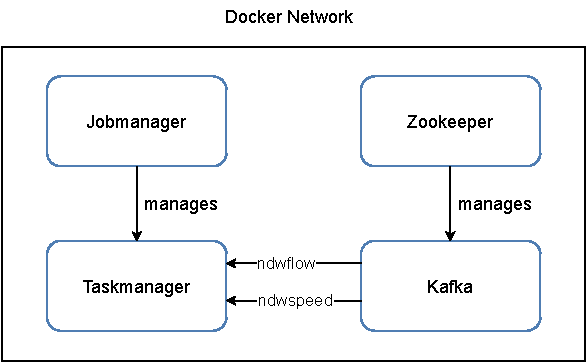
\includegraphics[width=\columnwidth]{fig/docker_setup.pdf}
    \caption[Setup of application containers inside the same docker network.]{ 
Setup of application containers inside the same docker network.
The kafka topics \emph{ndwflow} and \emph{ndwspeed} are consumed by the 
RMLStreamer job inside the Taskmanager.}
    \label{fig:docker_setup}
\end{figure}

\subsection{Metrics measurement}%
\label{sub:Metrics measurement}

CPU usage, throughput, memory, and latency exposed 
by Flink's Rest API, are constantly polled every 100ms by a 
Python script scraper.
CPU usage, throughput 
and memory usage are measured internally by Flink,
while latency measurement 
is implemented manually using Flink's Metrics API to more accurately measure the amount of 
time spent in the window by a record before being processed. 

The aforementioned metrics are averaged across the parallelized window operators.
Intersection over union (IOU) is used as the metric to measure the completeness
of the joined result generated by the windows.  


\subsubsection{CPU usage}%
\label{ssub:CPU usage}
For CPU usage, we measure Taskmanager's CPU usage, since it is 
the one responsible for executing the RMLStreamer code. 

\subsubsection{Throughput}%
\label{ssub:Throughput}
Throughput measurement is defined as the number of records processed by the 
window operator per second. 
It is measured at the output of the window operator, since we want to measure 
output performance of the window operators. 


\subsubsection{Memory usage}%
\label{ssub:Memory usage}
Due to limitation in granularity of measurement in Flink, 
JVM heap memory of the job is used to estimate the memory usage of window 
operator. We expect the memory usage by other operators in the job to be 
consistent and low across the different evaluation runs since they are stateless operators.

\subsubsection{Latency measurement}%
\label{ssub:Latency measurement}
We measure the latency by attaching a processing timestamp to the 
records before they enter the window. 
Once the records are processed and emitted after the join, the difference 
between the current processing time and the attached old processing time 
is taken as the \emph{latency} for the records. 

\subsubsection{Completeness measurement}%
\label{ssub:Completeness measurement}
To generate \emph{bounded} input data for 
the static mapping engine, we write the stored data from the topics 
into a file on disk. This input data is processed by RMLStreamer in bounded data 
processing mode to generate the \emph{complete} set of triples. 

The generated output triples from the evaluation of the windows, and the bounded data processing are 
used to calculate the IOU metric to measure the similarity between the two outputs.    



\subsection{Workload scenarios}
\label{sec:workload}
We evaluate our dynamic window implementation under different workload scenarios. 
These workloads are similar to the ones used in~\cite{evalution_of_spe} where relevant.

\subsubsection{Workload for latency measurement}
Measurement of the \emph{latency} caused only 
by the window implementations, requires the stream processing framework not to be 
stressed by significant \emph{throughput}. Thus, the Kafka broker 
publishes the records at a very low constant rate of around 400 messages per second for 
this workload.
We denote this as \emph{constant} stream rate in the paper. 

\subsubsection{Workload with periodic burst}
We evaluate our implementation for its ability to cope with unstable 
streaming data sources with varying velocity.
The workload has a constant low stream rate with an occasional 
burst of data. Therefore, 38 000 records will be published every 10 seconds which 
takes around 170ms to 180ms since the time taken to publish can deviate based on the 
load of the Kafka brokers.
We denote this as \emph{periodic} stream rate in the paper. 

\subsubsection{Workload for completeness}
We will use two stream rates, constant and periodic, 
to measure the \emph{completeness} of the results generated 
by the different windows.







\section{RESULTS AND DISCUSSION}%
\label{chap:Results and Discussion}

The workload evaluations are run multiple times for consistency of results. 
For each workload we give a brief overview of the performance gain 
achieved by the Dyanmic window. 

\subsection{Workload for latency measurement}%
\label{sec:Results Workload for latency measurement}
For latency, Tumbling window has a median value of 1915ms, 
with latency ranging from 1081ms to 2624ms (Figure~\ref{fig:constant_tumb_boxplot})
more than $10\times$ the lantency of Dynamic window, which has a median 
of 57 and ranging from 39 to 120ms (Figure~\ref{fig:constant_dynamic_boxplot}). 
Our improvement to fire the \emph{trigger} event whenever a
new record arrives inside the 
subwindow, allows 
Dynamic window to achieve sub second latency. 

Dynamic window has a 
steady throughput of around 17200 records per second whereas Tumbling window fluctuates between 
12500 and 12800 records per second before stabilizing at 12750 records per second (Figure~\ref{fig:constant_thorughput}). 
This is due to the adjustment of window sizes at the subwindow level, allowing Dynamic window to wait for more records 
with infrequent \emph{key} attribute in the stream, before evicting the subwindow. 
In contrast, Tumbling window 
always evicts the content of the window after 2 seconds without waiting for more 
records.

Relative memory usage of Dynamic window compared to Tumbling window 
is similar over the lifetime of the 
evaluation run (Figure~\ref{fig:constant_mem_diff}). 
Dynamic window causes infrequent \emph{spikes} in memory usage of over
100 MB more than Tumbling window at a certain point in the lifetime of evaluation. 
This can be attributed 
to the subwindows of Dynamic window growing larger due to low stream 
rate. However,
Dynamic window stabilizes to a more optimal 
window size, where it uses less memory than Tumbling windows. 
At worst case, it uses as much memory as Tumbling window does over the course of the evaluation. 

CPU usage is higher by around 7\% for Dynamic window since it requires extra processing of the calculation of metrics and 
it increases the throughput causing RMLStreamer to process more joined records.
(Figure~\ref{fig:constant_cpu}). 

\begin{figure}[htbp]
    \begin{subfigure}[b]{0.5\columnwidth}
        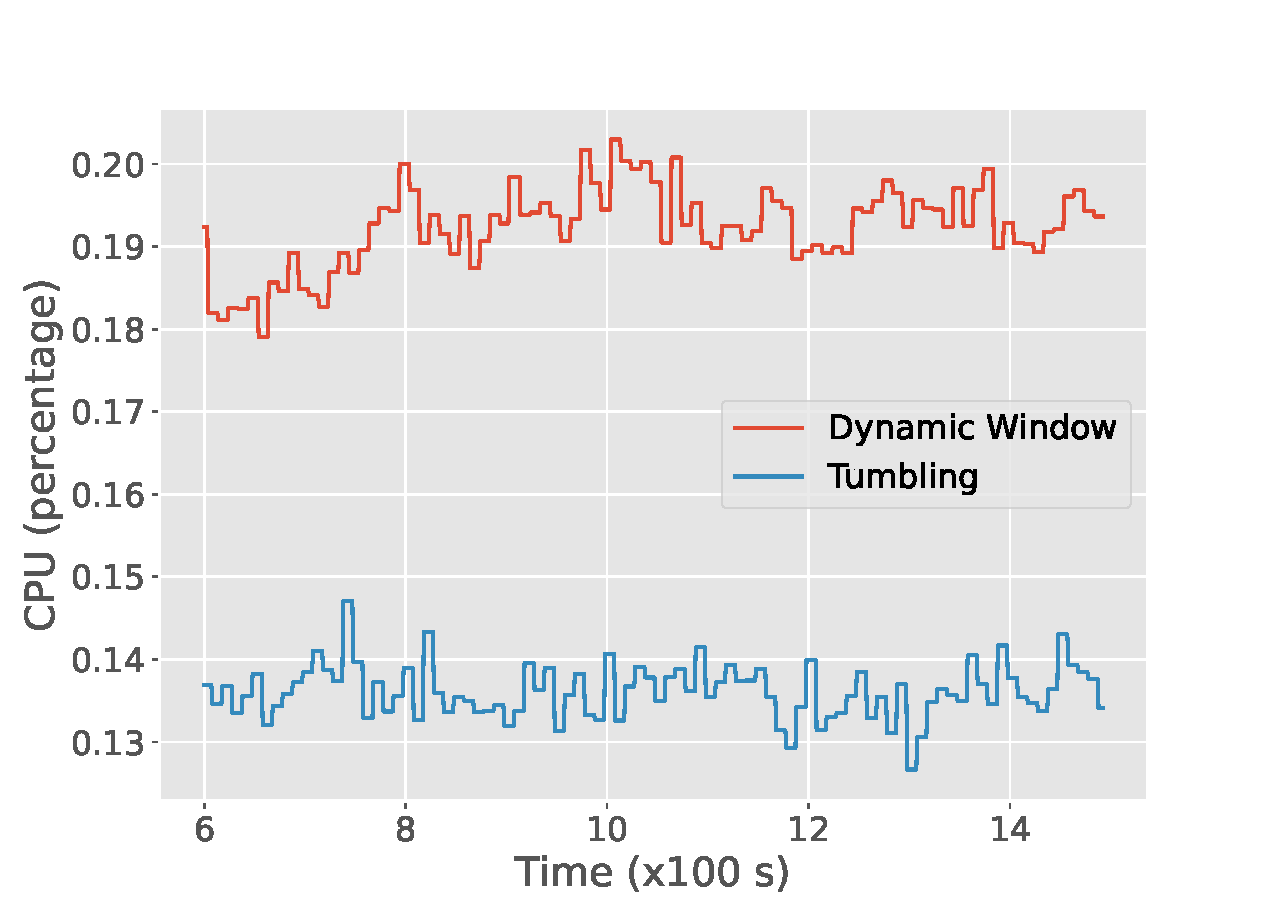
\includegraphics[width=\columnwidth]{fig/constant-rate/cpu_comparison.pdf}
        \caption{CPU usage}
        \label{fig:constant_cpu}
    \end{subfigure}
    \begin{subfigure}[b]{0.5\columnwidth}
        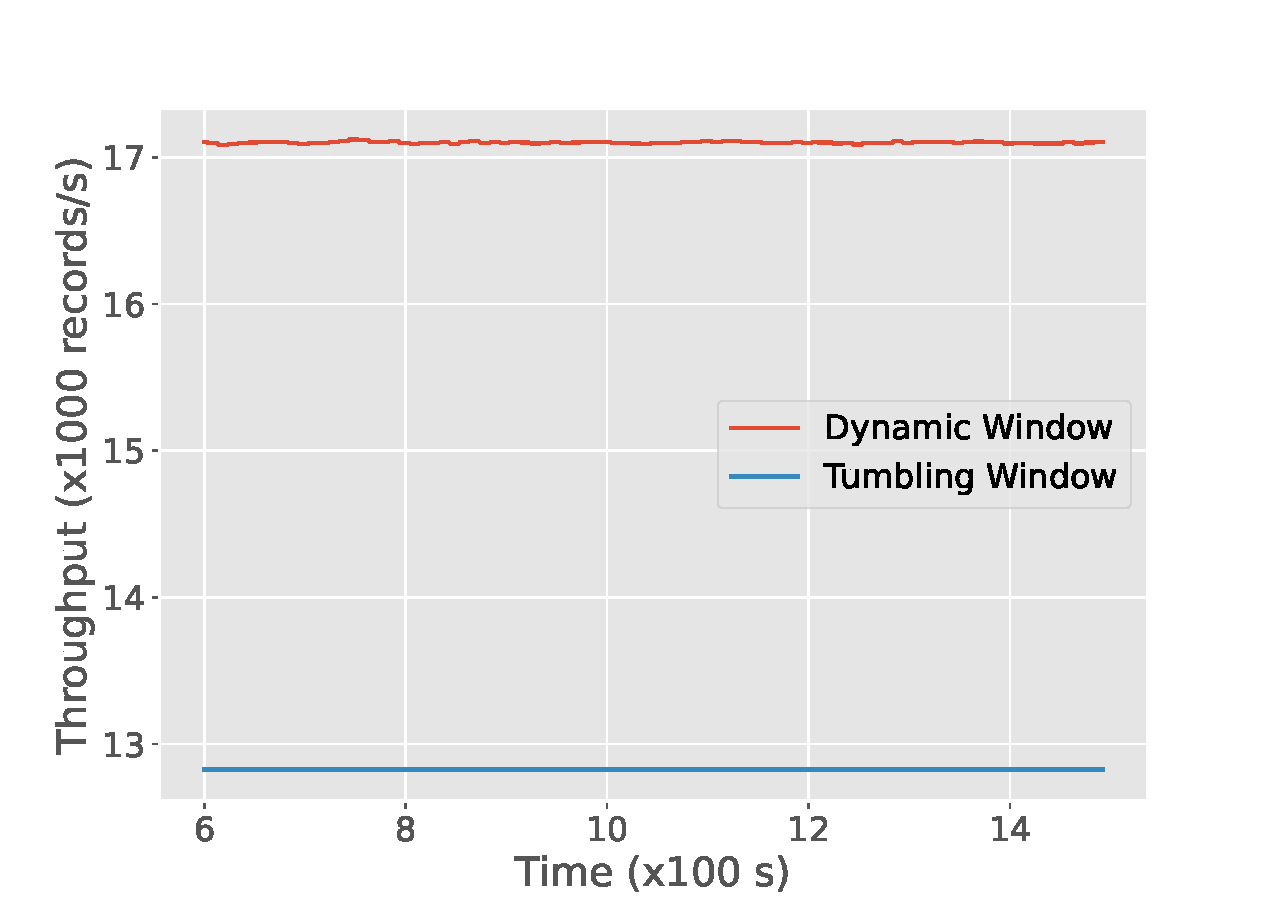
\includegraphics[width=\columnwidth]{fig/constant-rate/throughput_comparison.pdf}
        \caption{Throughput}
        \label{fig:constant_thorughput}
    \end{subfigure}
    %%
    \\
    \begin{subfigure}[b]{0.5\columnwidth}
        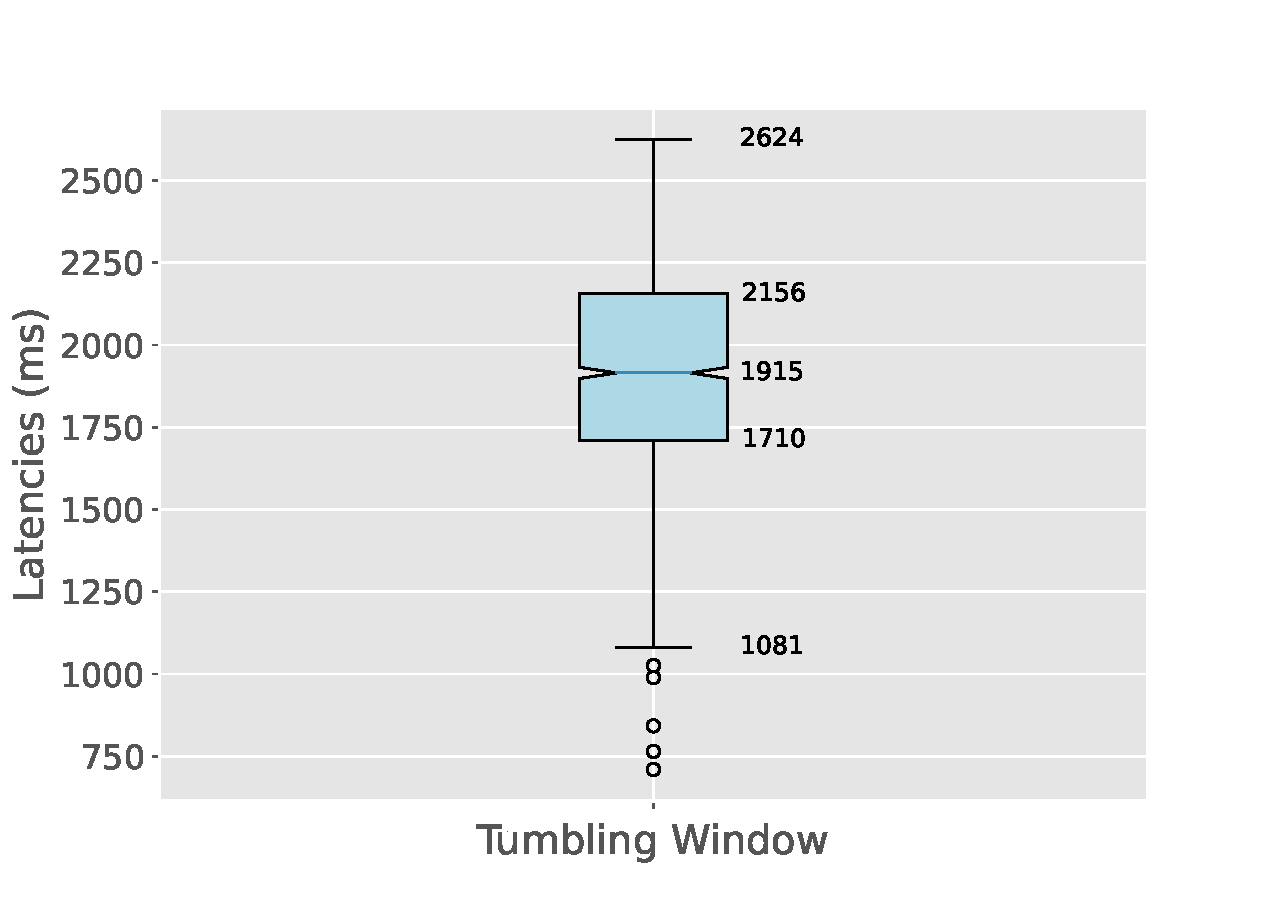
\includegraphics[width=\columnwidth]{fig/constant-rate/TumblingWindow_latency_boxplot.pdf}
        \caption{Tumbling latency}
        \label{fig:constant_tumb_boxplot}
    \end{subfigure}
    \begin{subfigure}[b]{0.5\columnwidth}
        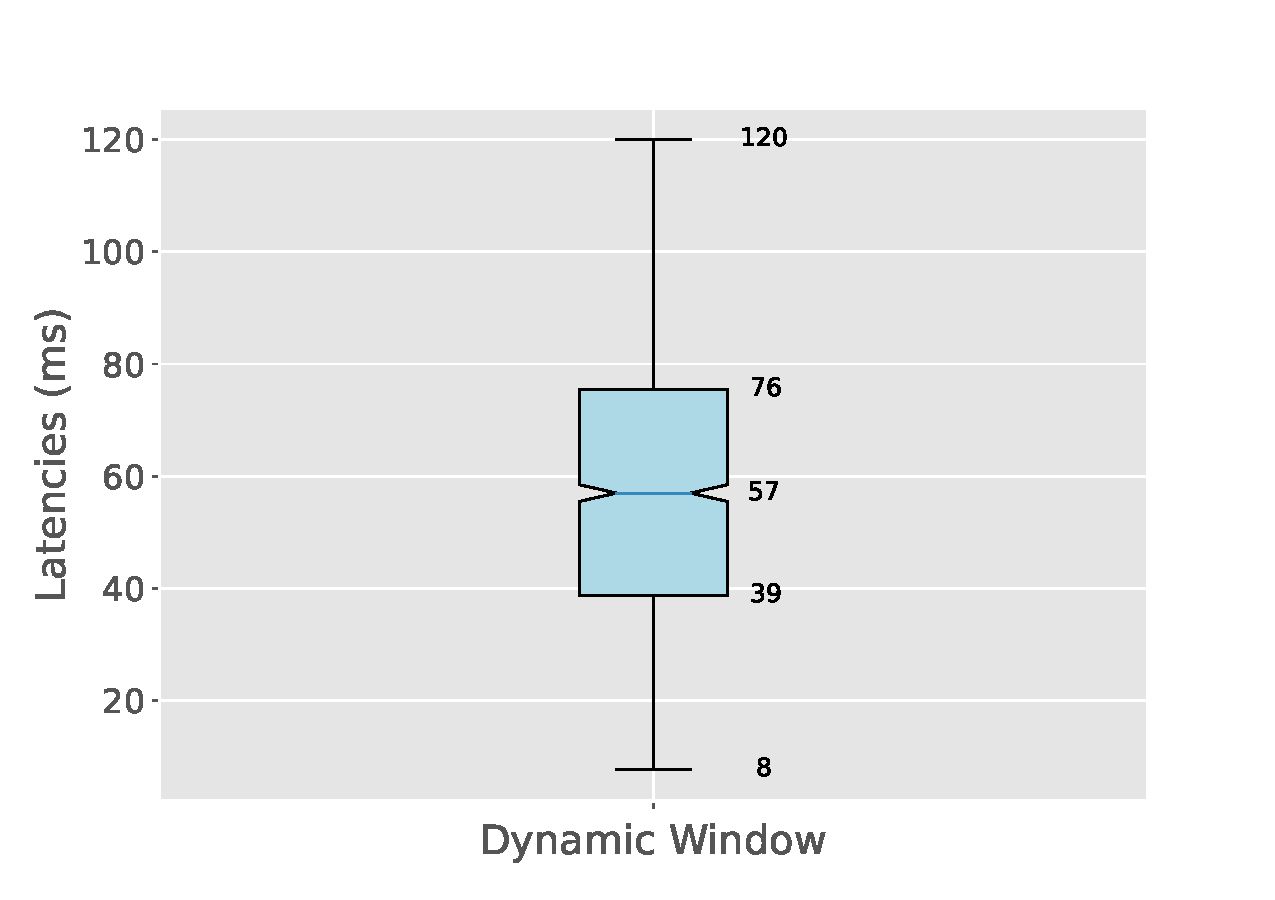
\includegraphics[width=\columnwidth]{fig/constant-rate/DynamicWindow_latency_boxplot.pdf}
        \caption{Dynamic latency}
        \label{fig:constant_dynamic_boxplot}
    \end{subfigure}
    % \\
    \\
    \begin{subfigure}[b]{\columnwidth}
        \centering
        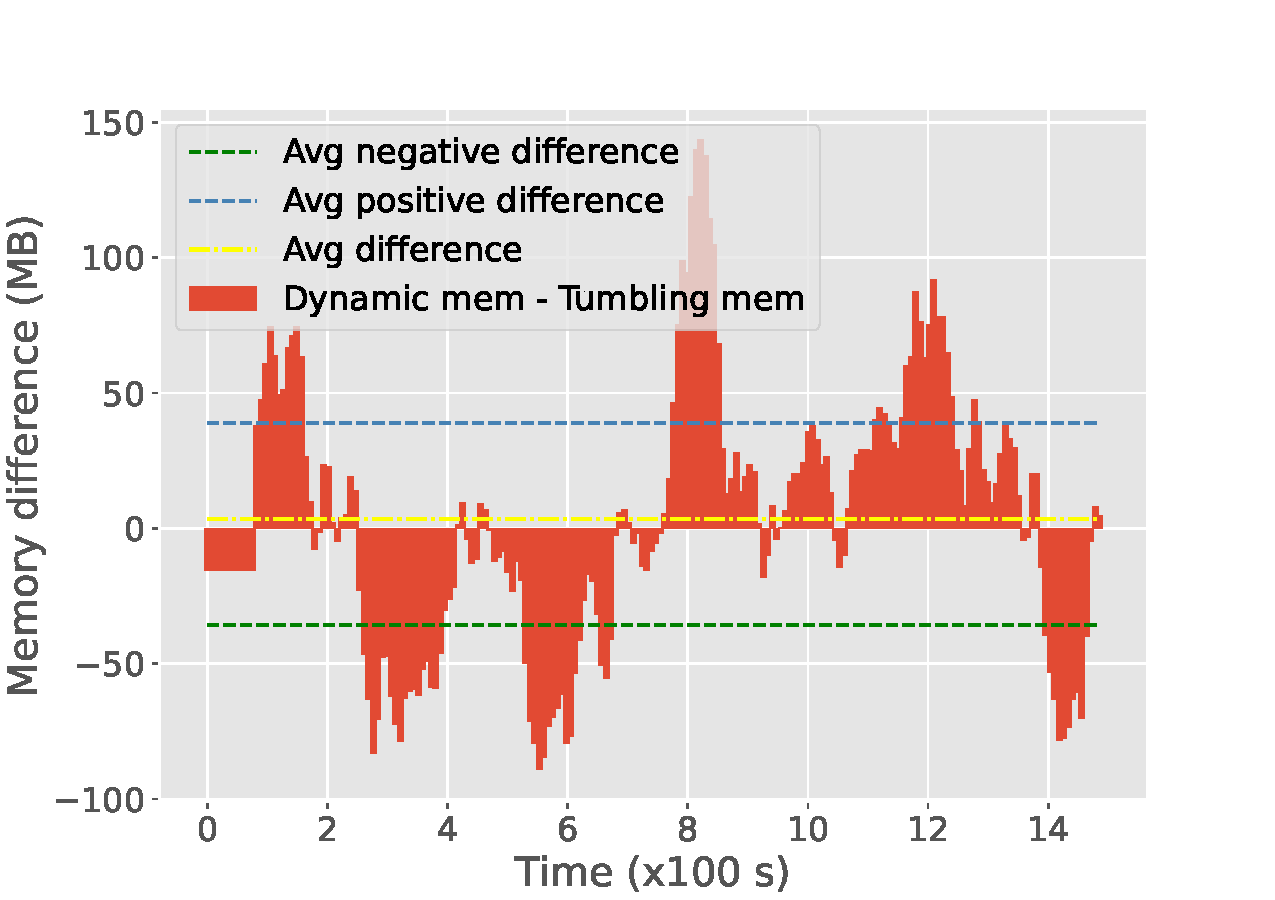
\includegraphics[width=0.5\columnwidth]{fig/constant-rate/mem_difference_bar.pdf}
        \caption{Relative difference in memory usage from the perspective of dynamic window}
        \label{fig:constant_mem_diff}
    \end{subfigure}

    \caption[Metrics measurements for latency workload.]
    {Metrics measurements for latency workload. Dynamic window performs 
    better in all measurements with the exception of CPU usage due to
overhead in dynamic adjustment of subwindow sizes.}%
    \label{fig:constant_measurement}
\end{figure}

\subsection{Workload for periodic burst}%
\label{sec:Results Workload for periodic burst}

Dynamic window still handles the periodic burst of data with lower latency 
than Tumbling window with latency in the range from 8ms to 1669ms
(Figure~\ref{fig:periodic_dynamic_boxplot}) compared to 
Tumbling window's range from 891ms to 3904ms 
(Figure~\ref{fig:periodic_tumb_boxplot}) which is double the latency 
measured for Dynamic window.
However, there is a temporary increase in latency at the beginning 
(Figure~\ref{fig:periodic_dynamic_lineplot}), 
when the burst of data arrives at every 10th second. 
This is due to the initial size of 2s subwindows for the initial low stream rate of 400 records per second. 
The subwindow sizes start to grow \textbf{larger} than 2s because of the low stream rate. 
The increase in the subwindow size results in the 
window having more records to join; causing a back pressure to form and latency to increase.  
This results in a positive skew in the latency distribution for Dynamic window (Figure~\ref{fig:periodic_dynamic_boxplot}). 
However, Dynamic window eventually manages to shorten the subwindow sizes as an
adaptation to the periodic burst of data until it achieves sub second latency again.


The throughput of both windows increased as expected.
Moreover, we observe a bigger difference in the throughput between the 
two windows of about 7000 records per second 
(Figure~\ref{fig:periodic_throughput}). However, the
constant and flat throughput measurement does not agree 
with the results of ~\cite{evalution_of_spe} where there are clear "spikes" in 
the throughput measurement which correspond to the periodic burst 
of records processed by the windows. 
We ran our evaluation as part of the whole RMLStreamer pipeline, causing 
a slight back pressure 
leading to a high and flat throughput measurement. 

CPU usage difference of the windows, is similar to the 
workload for latency measurement with relative increase for 
burst data procesing
(Figure~\ref{fig:periodic_cpu}). 

Surprisingly,
Dynamic window uses 
about 10 MB less memory on average than Tumbling window during the lifetime of the evaluation (Figure~\ref{fig:periodic_mem_diff}). 
The initial memory usage for Dynamic window is about 100 MB higher than for 
Tumbling window due to the long window growth 
caused by the low stream rate. However, once 
the dynamic adjustment of subwindow kicks in, reducing the memory usage.


\begin{figure}
    \begin{subfigure}[b]{0.5\columnwidth}
        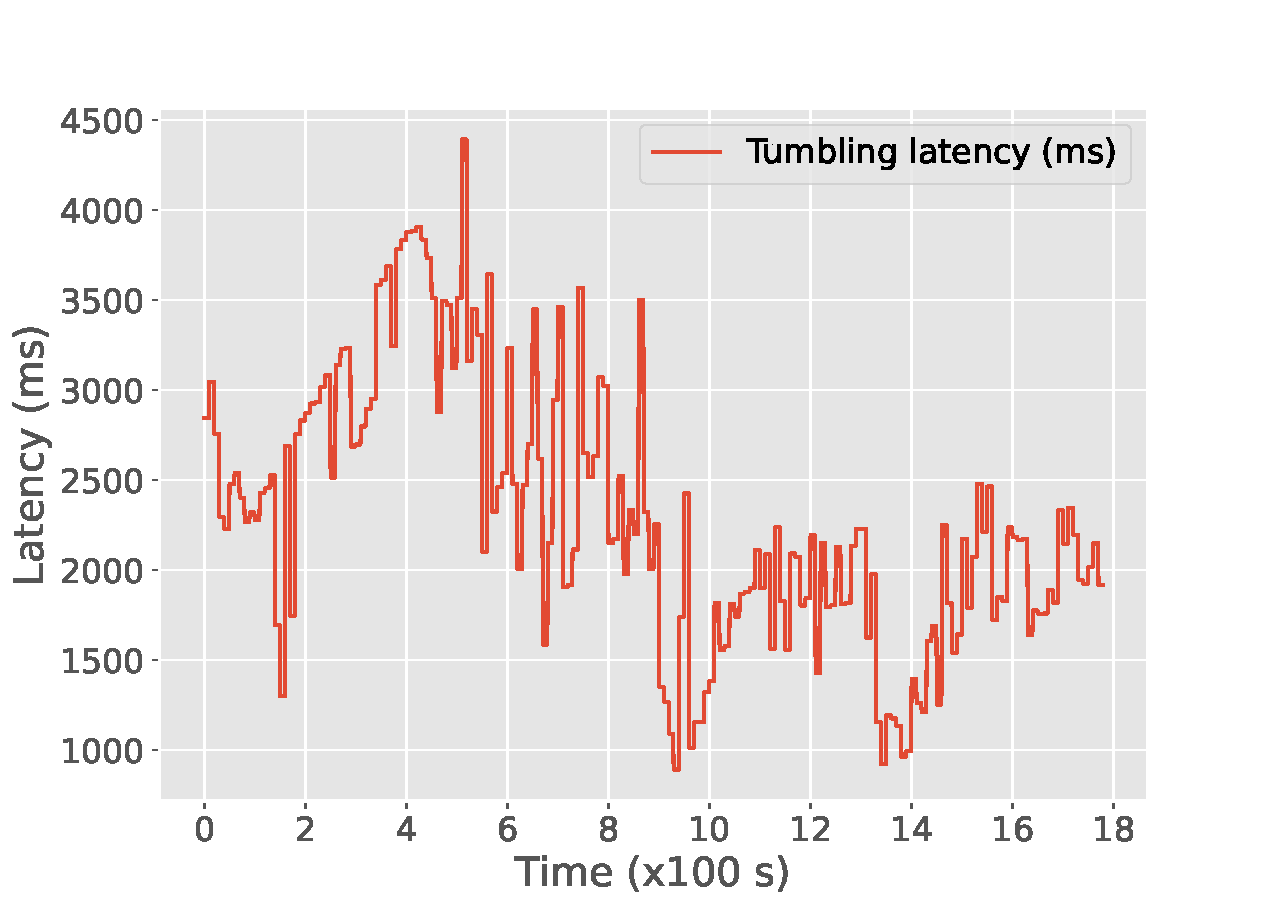
\includegraphics[width=\columnwidth]{fig/periodic/Tumbling_latency_lineplot.pdf}
        \caption{Tumbling latency }
        \label{fig:periodic_tumbling_lineplot}
    \end{subfigure}
    \begin{subfigure}[b]{0.5\columnwidth}
        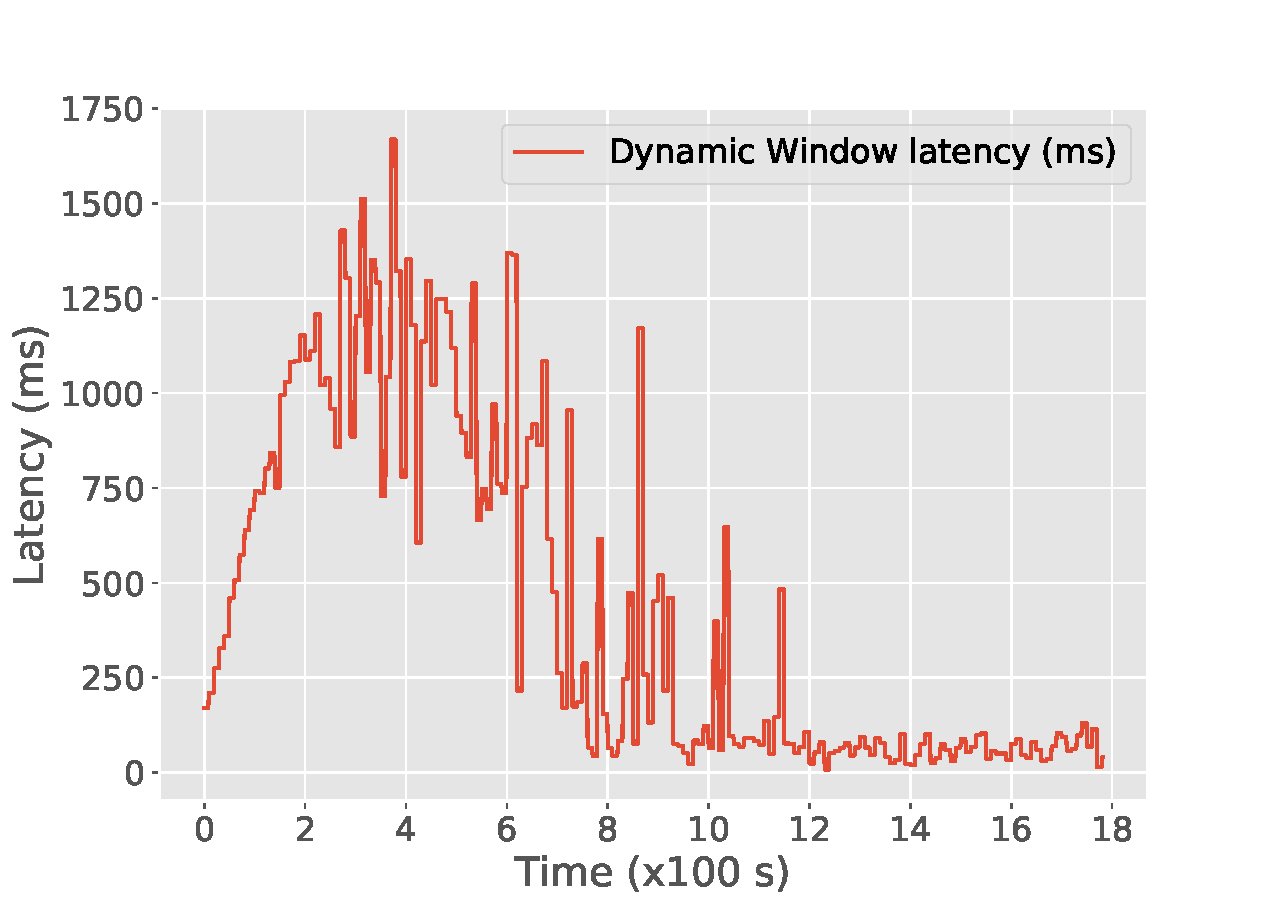
\includegraphics[width=\columnwidth]{fig/periodic/DynamicWindow_latency_lineplot.pdf}
        \caption{Dynamic latency }
        \label{fig:periodic_dynamic_lineplot}
    \end{subfigure}
    \caption{Latency measurement of periodic workload over the lifetime of evaluation}
    \label{fig:periodic_latency_lineplot}
\end{figure}

\begin{figure}
    \begin{subfigure}[b]{0.5\columnwidth}
        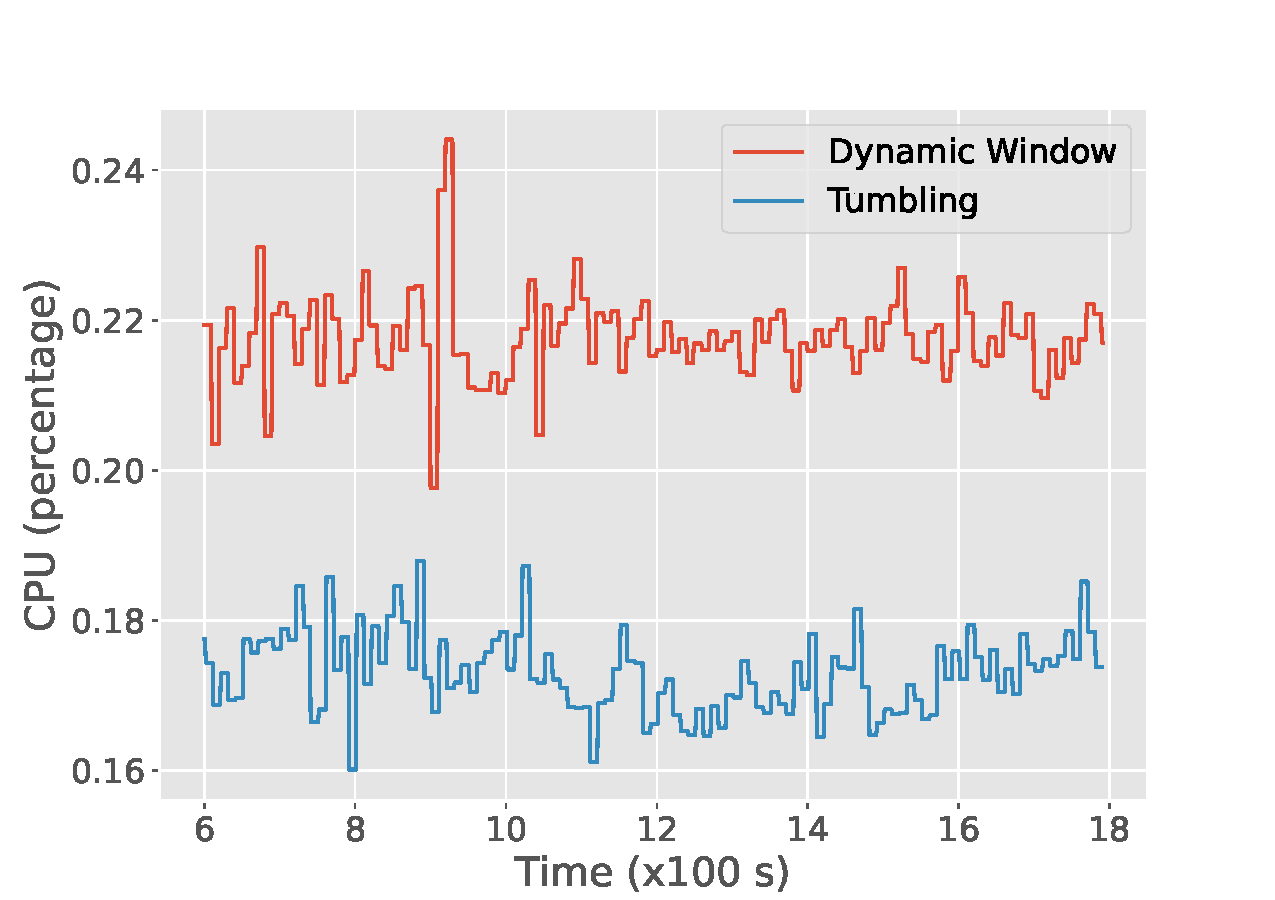
\includegraphics[width=\columnwidth]{fig/periodic/cpu_comparison.pdf}
        \caption{CPU usage}
        \label{fig:periodic_cpu}
    \end{subfigure}
    \hfill 
    \begin{subfigure}[b]{0.5\columnwidth}
        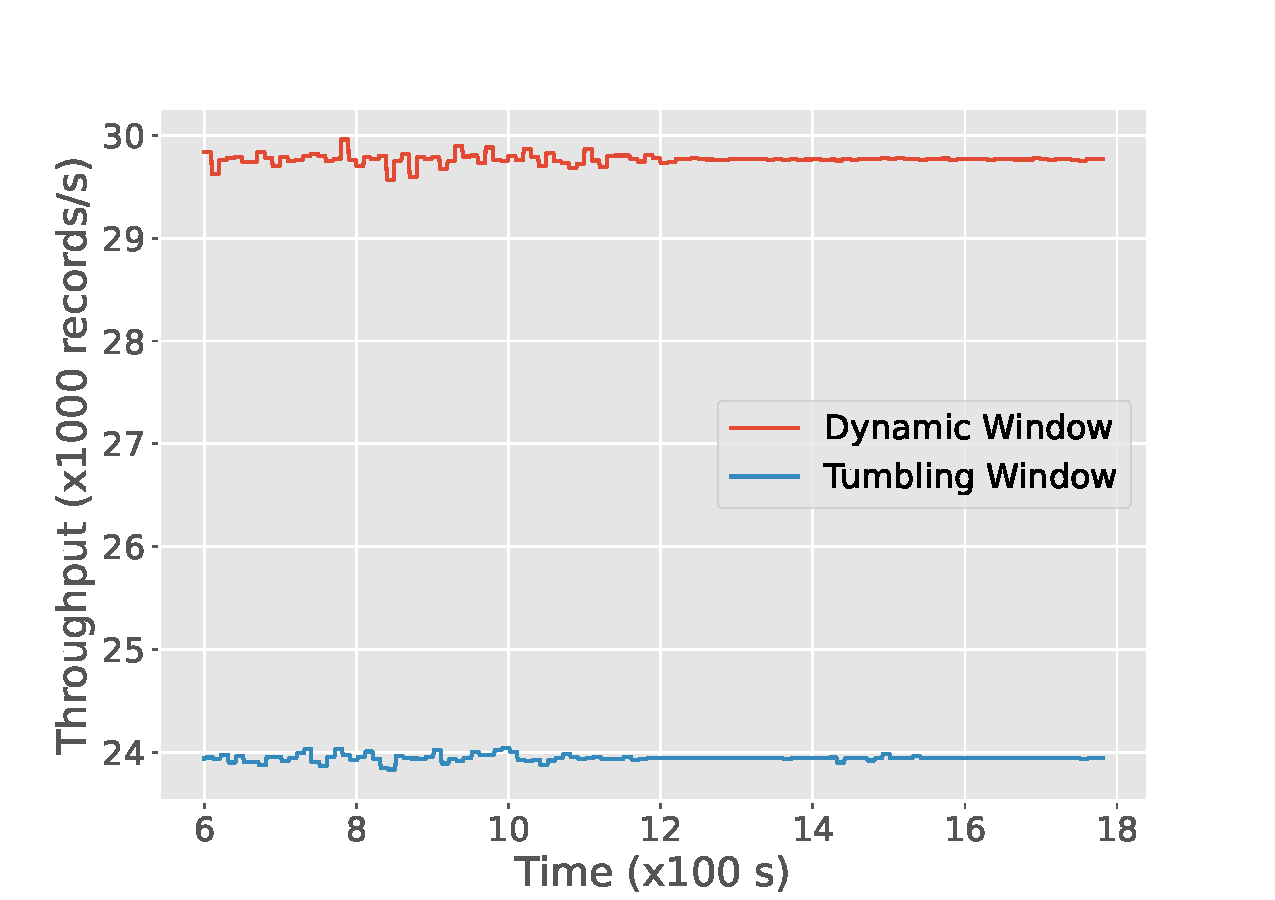
\includegraphics[width=\columnwidth]{fig/periodic/throughput_comparison.pdf}
        \caption{Throughput }
        \label{fig:periodic_throughput}
    \end{subfigure}
    %%
    \begin{subfigure}[b]{0.5\columnwidth}
        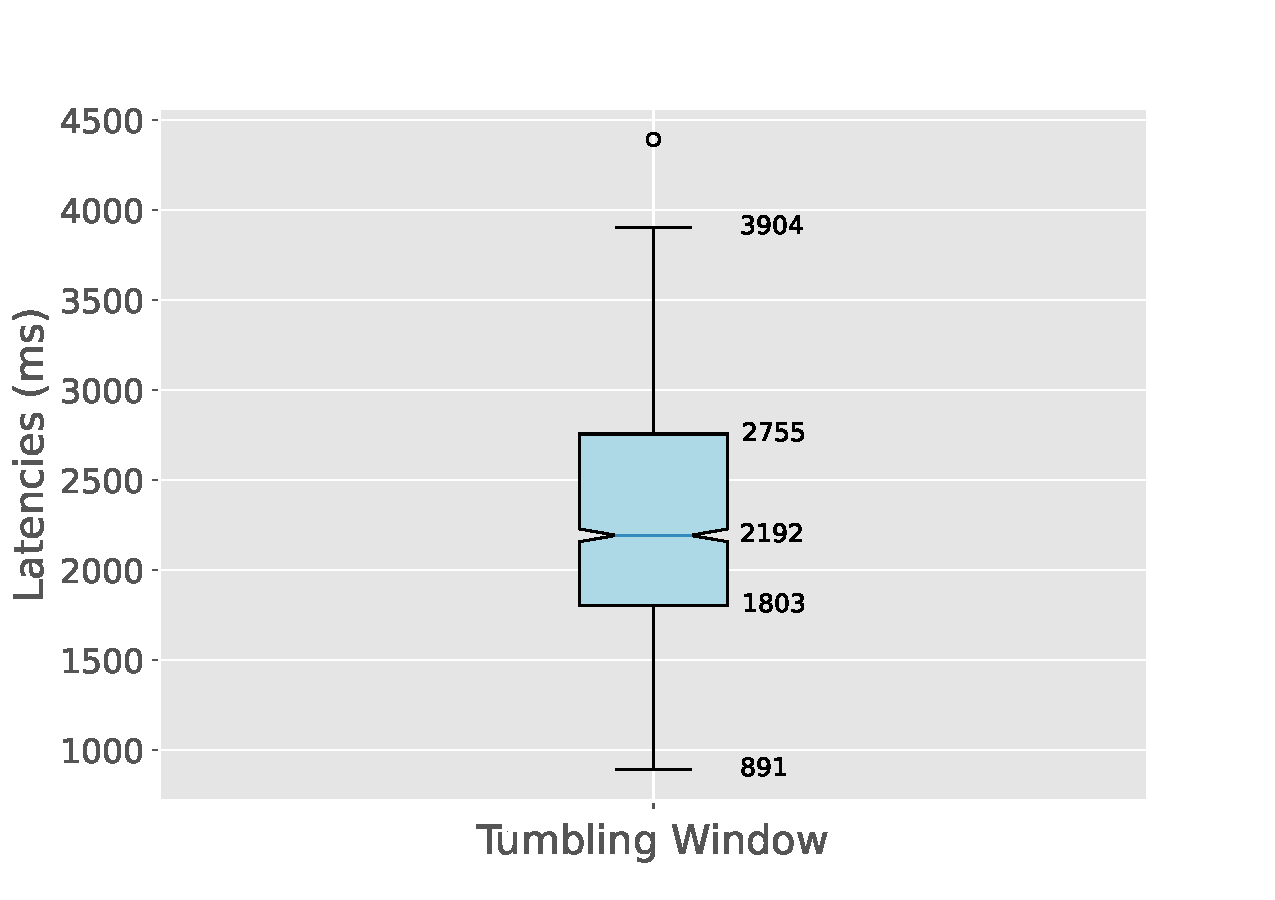
\includegraphics[width=\columnwidth]{fig/periodic/TumblingWindow_latency_boxplot.pdf}
        \caption{Tumbling latency distribution}
        \label{fig:periodic_tumb_boxplot}
    \end{subfigure}
    \hfill 
    \begin{subfigure}[b]{0.5\columnwidth}
        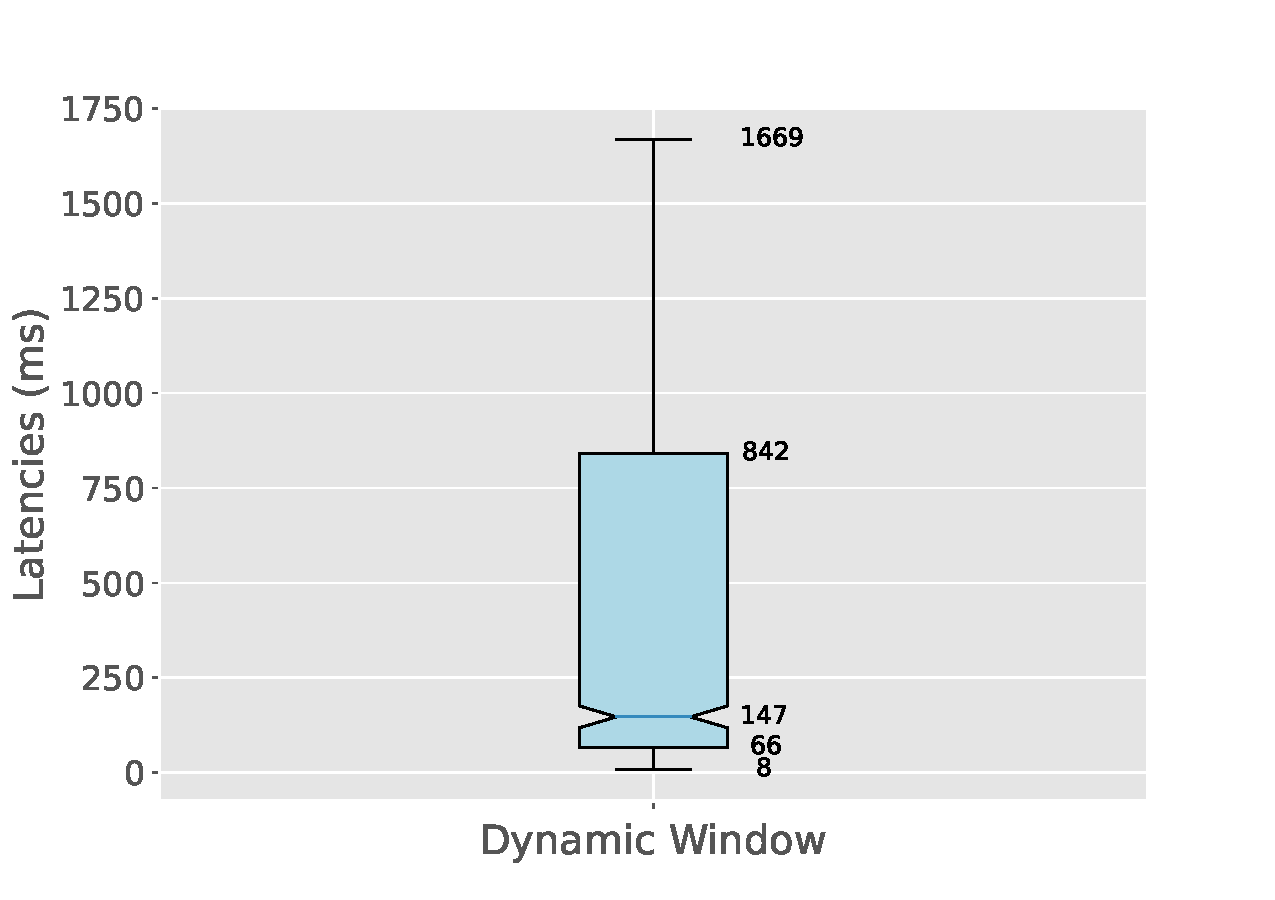
\includegraphics[width=\columnwidth]{fig/periodic/DynamicWindow_latency_boxplot.pdf}
        \caption{Dynamic latency distribution}
        \label{fig:periodic_dynamic_boxplot}
    \end{subfigure}
    % 
    \begin{subfigure}[b]{\columnwidth}
        \centering
        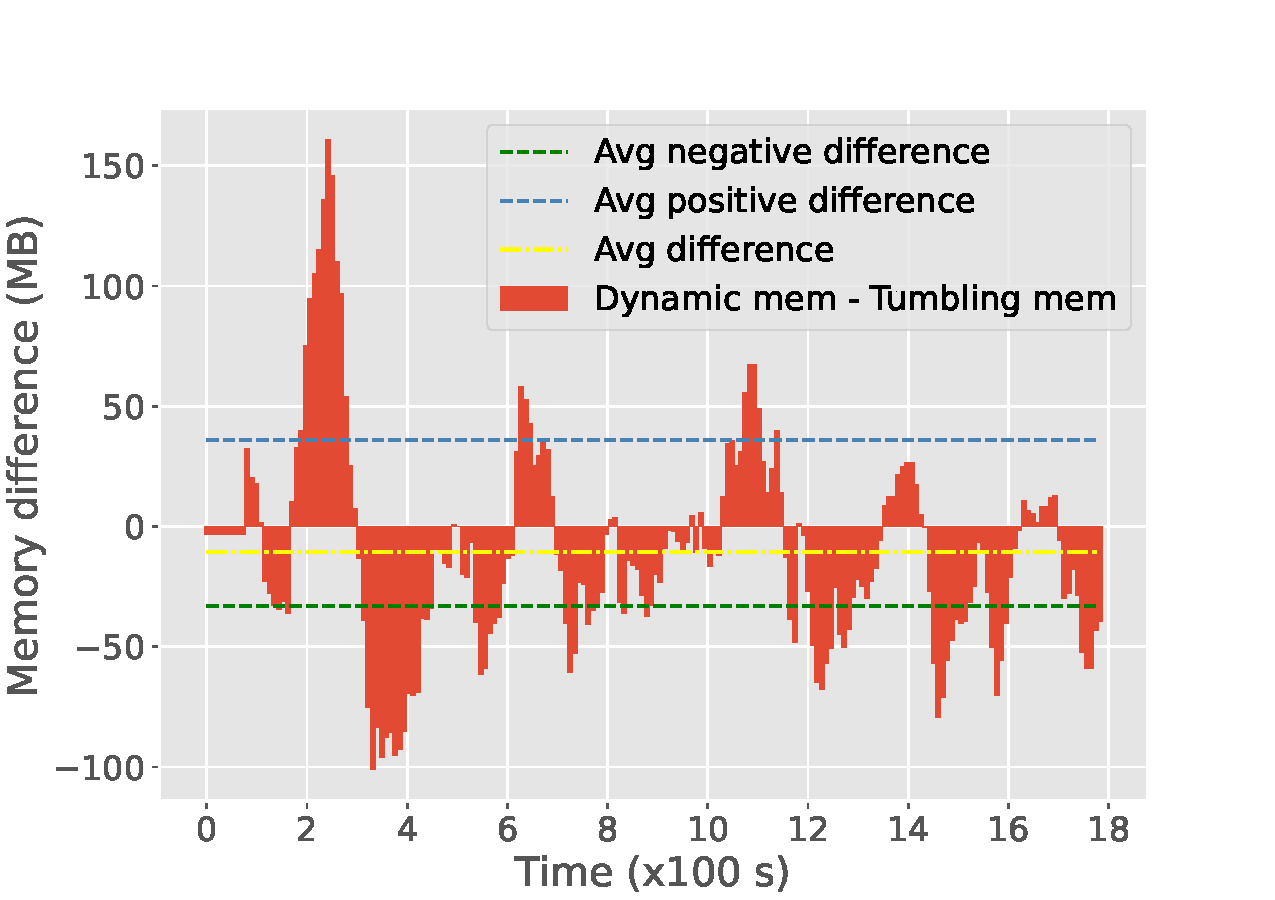
\includegraphics[width=0.5\columnwidth]{fig/periodic/mem_difference_bar.pdf}
        \caption{Relative difference in memory usage from the perspective of dynamic window}
        \label{fig:periodic_mem_diff}
    \end{subfigure}

    \caption[Metrics measurements for periodic workload]
    {Metrics measurements for periodic workload. Dynamic window 
    has lower memory usage on average than Tumbling window for
periodic workload. }%
    \label{fig:periodic_measurement}
\end{figure}

\subsection{Workload for completeness measure}%
\label{sec:Workload for completeness measure}

From the results in Table~\ref{tab:dynamic_completeness}, and 
Table~\ref{tab:tumbling_completeness}, we conclude that Dynamic window 
outperforms Tumbling window in terms of generating a more \emph{complete} output. 
Dynamic window has an IOU score of \textbf{1} for constant low stream rate
due to the subwindow sizes growing large 
enough to accommodate all the required records, to generate the \emph{complete} set 
of output. In contrast, Tumbling window scores only \textbf{0.749}, leading to 
a conclusion that a window size of 2s is not enough to process the low stream rate 
of the evaluation data. 

Similarly for periodic burst input, Dynamic window outperforms Tumbling window with a
score of \textbf{0.982} whereas Tumbling window only scores \textbf{0.780}. The high IOU 
score of Dynamic window is due to its ability  
to adapt to the changing stream rate to hold enough 
records for maximal joined output generation.


\begin{table}[htbp]
    \centering
    \resizebox{0.5\columnwidth}{!}{%
\begin{tabular}{|r|r|}
\hline
\multicolumn{1}{|c|}{Stream rate} & \multicolumn{1}{c|}{\textbf{IOU score}} \\ \hline
Constant rate                                              & \textbf{1}                              \\ \hline
Periodic burst                                        & \textbf{0.982}                          \\ \hline
\end{tabular}%
}
\caption{Dynamic window's completeness measurement.}
\label{tab:dynamic_completeness}
\end{table}

\begin{table}[htbp]
    \centering
    \resizebox{0.5\columnwidth}{!}{%
\begin{tabular}{|r|r|}
\hline
\multicolumn{1}{|c|}{Stream rate} & \multicolumn{1}{c|}{\textbf{IOU score}} \\ \hline
Constant rate       & \textbf{0.749}                              \\ \hline
Periodic burst      & \textbf{0.780}                          \\ \hline
\end{tabular}%
}
\caption{Tumbling window's completeness measurement. }
\label{tab:tumbling_completeness}
\end{table}


\subsection{Summary}%
\label{sec:Result Summary}

In summary, these results show that our implementation of Dynamic window 
provides lower latency, higher throughput, and a more complete 
output than Tumbling window for both 
workloads of constant stream rate, and unstable periodic burst stream rate.

Although memory usage dropped in the workload with periodic burst rate, we 
could not confidently conclude that the Dynamic window effectively used less memory
on average than Tumbling window. The measurement was based on the heap memory of the 
whole evaluation job, not just the window operator. Therefore, there is a need for a 
more precise measurement of memory usage. 

The results for throughput also deviate from those reported by Van Dongen and Van den Poel(2020)~\cite{evalution_of_spe}. 
This is due to the fact that we ran the evaluation using the whole pipeline of RMLStreamer. This incurs some back pressure from the mapping stage, 
causing the throughput of the join stage to stay constant and flat.    

Overall, we could conclude that Dynamic windowing is viable to replace the fixed size 
windows. Especially in use 
cases, where windows are not required to be of fixed size with variable stream rate.  


\section{Conclusion and Future Works}%
\label{chap:Conclusion and Future Works}

In this paper, we have presented an approach for Dynamic window 
which adapts its window size according to the stream rate of the 
input data sources. We introduced a simple heuristic to adapt 
window sizes dynamically without huge memory or computation overhead. 

We implemented our Dynamic window on top of the existing RMLStreamer, 
to evaluate its performance under a realistic processing environment. 
We adapted the benchmark framework as stated in~\cite{evalution_of_spe} to 
accurately evaluate the performance of our implementation against the 
standard fixed size Tumbling window. 

The results show that our implementation 
of Dynamic window performs better than Tumbling window in terms of 
latency, throughput, and completeness with only a slight 
increase in CPU usage. Even though we could not confidently conclude that
memory usage is lower in Dynamic window, our preliminary results indicate 
that it performs the same as Tumbling window in the worst-case scenario.

Therefore, there are still areas of improvement to be made.
On the evaluation side, we could further increase 
the precision of our memory measurement by only counting the number of records
residing in the windows at any moment instead of the whole JVM heap of the RMLStreamer job. 
Furthermore, the evaluation could be done in the same benchmark pipelines as in~\cite{evalution_of_spe} 
to further evaluate the Dynamic window performance in a general stream processing case.
Improvements on our dynamic approach could be achieved by allowing users to 
define other statistical approaches
to better calculate the threshold for adapting the window sizes. 



%%%%%%%%%%%%%%%%%%%%%%%%%%%%%%%%%%%%%%%%%%%%%%%%%%%%%%%%%%%%%%%%%%%%%%%%%%%%%%%%

\printbibliography

\end{document}
